\documentclass[border=4pt,12pt]{standalone}
% House style for redrawn exam diagrams (diagram-v4: 0.4pt lines, filled -latex arrows, fine dashes; stipple and hatching drawn as real dots/lines (no PDF/SVG patterns, so they render in every browser and at any scale); transparent background). Every figure \input's this.
\usepackage{amsmath,amssymb}
\usepackage{txfonts}
\usepackage{pdfrender,xcolor}
% \halo{text}: label on shading. The shading stops just around each letter's outline (a thin knock-out that follows the
% glyphs, like the papers' typesetting), never a box. Owner: "I don't want a box around the text".
\newcommand{\halo}[1]{\leavevmode\rlap{\pdfrender{TextRenderingMode=2,LineWidth=2.2pt,LineJoinStyle=1,StrokeColor=white,FillColor=white}#1}#1}
\usepackage{tikz,pgfplots}
\pgfplotsset{compat=1.18}
\usetikzlibrary{arrows.meta,calc,angles,quotes,patterns,patterns.meta,intersections,positioning,decorations.markings,shapes.geometric}
% Stipple and hatching are drawn as actual dots / lines clipped to the region (path picture), NOT as pattern fills:
% SVG <pattern> fills vanish or blur when browsers scale the image, so the owner could not see the shading.
% Each dot is a 0.72pt square (keeps SVGs small; reads as a dot at print size). Dots sit on one global staggered grid, so neighbouring regions line up.
\makeatletter
\newdimen\ex@x \newdimen\ex@y \newdimen\ex@xa \newdimen\ex@ya \newdimen\ex@xb \newdimen\ex@yb \newcount\ex@row
\def\exam@stipplecolor{black!75}\def\exam@dotr{0.42pt}\def\exam@dotgap{2.5}
\def\ex@rowdots{\ifdim\ex@x<\ex@xb \pgfpathrectangle{\pgfqpoint{\dimexpr\ex@x-0.36pt\relax}{\dimexpr\ex@y-0.36pt\relax}}{\pgfqpoint{0.72pt}{0.72pt}}\advance\ex@x by \exam@dotgap pt\relax\expandafter\ex@rowdots\fi}
\def\exam@stipple{%
  \pgftransformreset% dots are sized in real points even inside scaled pictures
  \pgfpointanchor{path picture bounding box}{south west}\ex@xa=\pgf@x \ex@ya=\pgf@y
  \pgfpointanchor{path picture bounding box}{north east}\ex@xb=\pgf@x \ex@yb=\pgf@y
  \pgfsetfillcolor{\exam@stipplecolor}\pgfmathsetmacro\ex@h{\exam@dotgap/2}%
  \pgfmathtruncatemacro\ex@r{floor(\ex@ya/\ex@h)-1}\ex@row=\ex@r\relax
  \ex@y=\ex@r\dimexpr\ex@h pt\relax
  \loop\ifdim\ex@y<\ex@yb
    \pgfmathtruncatemacro\ex@c{floor(\ex@xa/\exam@dotgap)-1}\ex@x=\ex@c\dimexpr\exam@dotgap pt\relax
    \ifodd\ex@row \advance\ex@x by \ex@h pt\fi
    \ex@rowdots
    \advance\ex@y by \ex@h pt \advance\ex@row by 1
    \ifnum\numexpr\ex@row-(\ex@row/4)*4\relax=0 \pgfusepath{fill}\fi% flush every 4 rows: bounded TeX memory, few clip copies in the SVG
  \repeat\pgfusepath{fill}}
\newdimen\ex@d
\def\exam@hatch#1{% #1 = 1 for /, -1 for \ ; lines 45 degrees, 3pt apart
  \pgftransformreset
  \pgfpointanchor{path picture bounding box}{south west}\ex@xa=\pgf@x \ex@ya=\pgf@y
  \pgfpointanchor{path picture bounding box}{north east}\ex@xb=\pgf@x \ex@yb=\pgf@y
  \ex@d=\dimexpr\ex@yb-\ex@ya\relax \ex@x=\dimexpr\ex@xa-\ex@d\relax
  \loop\ifdim\ex@x<\ex@xb
    \ifnum#1>0 \pgfpathmoveto{\pgfqpoint{\ex@x}{\ex@ya}}\pgfpathlineto{\pgfqpoint{\dimexpr\ex@x+\ex@d\relax}{\ex@yb}}%
    \else \pgfpathmoveto{\pgfqpoint{\ex@x}{\ex@yb}}\pgfpathlineto{\pgfqpoint{\dimexpr\ex@x+\ex@d\relax}{\ex@ya}}\fi
    \advance\ex@x by 4.24pt
  \repeat
  \pgfsetlinewidth{0.4pt}\pgfsetstrokecolor{black}\pgfusepath{stroke}}
\def\examstipple{\exam@stipple}\def\examhatch{\exam@hatch}\def\examsetstipplecolor#1{\def\exam@stipplecolor{#1}}\def\examsetdotgap#1{\def\exam@dotgap{#1}}
\makeatother
% (legacy pattern kept for old files)
% staggered stipple like the NESA papers' dotted shading
\pgfdeclarepatternformonly{exam stipple}{\pgfpointorigin}{\pgfqpoint{2.2pt}{2.2pt}}{\pgfqpoint{2.2pt}{2.2pt}}{%
  \pgfpathcircle{\pgfqpoint{0.55pt}{0.55pt}}{0.42pt}\pgfpathcircle{\pgfqpoint{1.65pt}{1.65pt}}{0.42pt}\pgfusepath{fill}}
\tikzset{
  every picture/.style={line width=0.6pt, >={Latex[length=2mm,width=1.3mm]}},
  curve/.style={line width=0.6pt},
  open arrow/.style={-{Latex[length=2mm,width=1.3mm]}},  % owner: filled -latex heads everywhere, no open chevrons
  aux/.style={dash pattern=on 2pt off 1.5pt, line width=0.6pt},
  shade/.code={\def\exA{#1}\def\exB{none}\ifx\exA\exB\else\pgfkeysalso{fill=black!18}\fi},
  shade/.default=on,
  shade dots/.style={fill=none, path picture={\examstipple}},
  stipple color/.code={\examsetstipplecolor{#1}},
  stipple gap/.code={\examsetdotgap{#1}},
  shade dense dots/.style={fill=none, stipple gap=1.6, path picture={\examstipple}},
  shade hatch/.style={fill=none, path picture={\examhatch{1}}},
  shade hatch reverse/.style={fill=none, path picture={\examhatch{-1}}},
  shade solid/.style={fill=black},
  pt/.style={circle, fill, inner sep=1.1pt},
  open pt/.style={circle, draw, fill=white, inner sep=1.1pt},
}
\pgfplotsset{
  exam axes/.style={axis lines=middle, axis line style={->}, xlabel={$x$}, ylabel={$y$},
    xlabel style={anchor=west}, ylabel style={anchor=south}, tick label style={font=\small},
    every axis plot/.append style={line width=0.6pt, black}, samples=200, clip=false,
    enlargelimits=false, axis on top},
}

\begin{document}
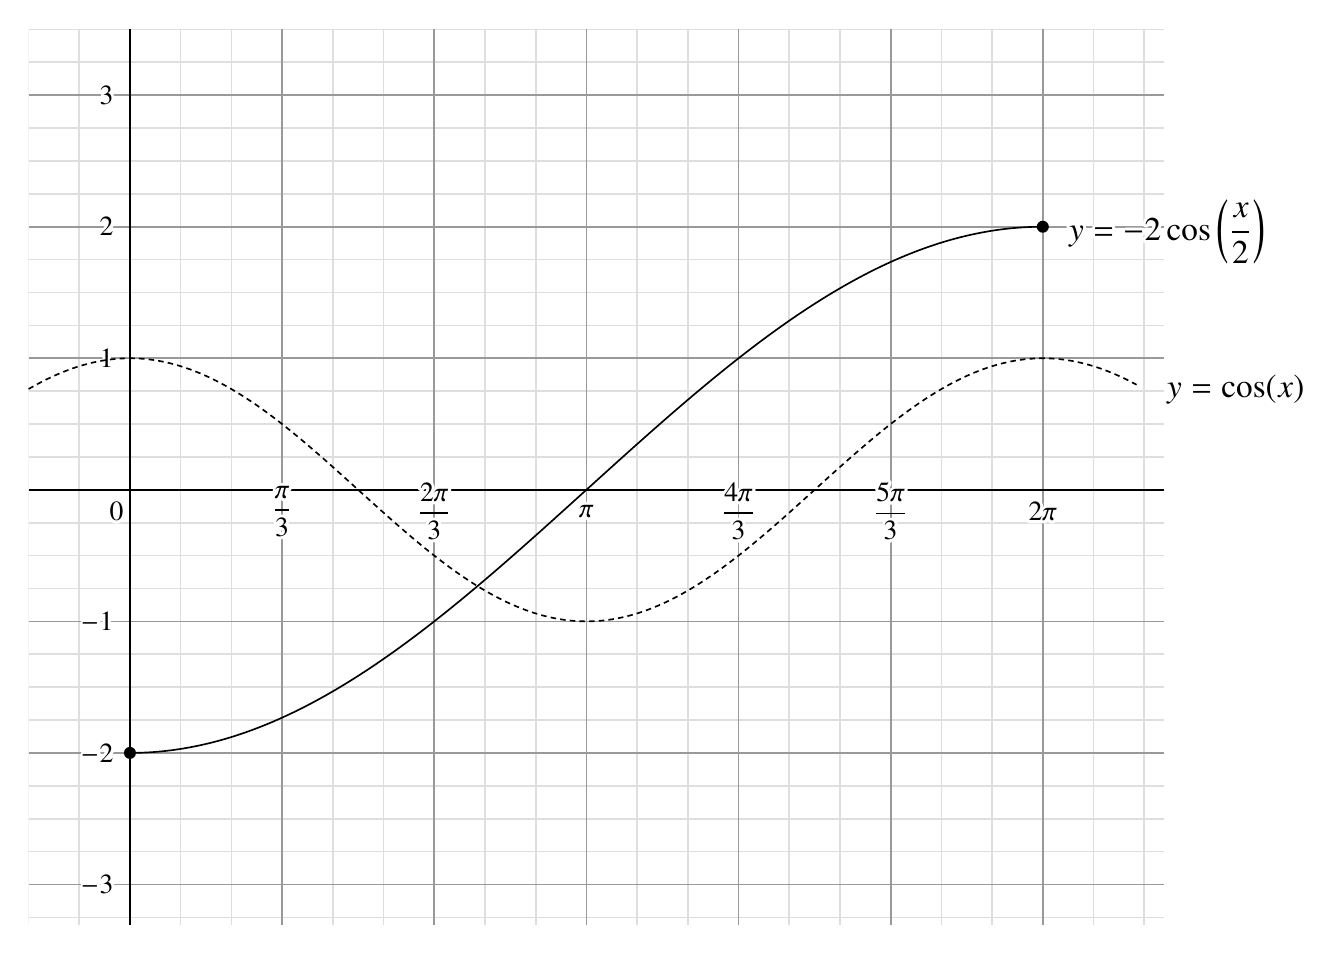
\begin{tikzpicture}[x=0.0127cm,y=-0.0127cm,every node/.style={font=\fontsize{10}{12}\selectfont}]
\begin{scope}\clip (9,8) rectangle (1145,905);
\draw[black!13] (9.0,8) -- (9.0,905);
\draw[black!13] (59.8,8) -- (59.8,905);
\draw[black!13] (161.2,8) -- (161.2,905);
\draw[black!13] (212.0,8) -- (212.0,905);
\draw[black!13] (313.4,8) -- (313.4,905);
\draw[black!13] (364.2,8) -- (364.2,905);
\draw[black!13] (465.6,8) -- (465.6,905);
\draw[black!13] (516.4,8) -- (516.4,905);
\draw[black!13] (617.8,8) -- (617.8,905);
\draw[black!13] (668.6,8) -- (668.6,905);
\draw[black!13] (770.0,8) -- (770.0,905);
\draw[black!13] (820.8,8) -- (820.8,905);
\draw[black!13] (922.2,8) -- (922.2,905);
\draw[black!13] (973.0,8) -- (973.0,905);
\draw[black!13] (1074.4,8) -- (1074.4,905);
\draw[black!13] (1125.2,8) -- (1125.2,905);
\draw[black!13] (1226.6,8) -- (1226.6,905);
\draw[black!13] (1277.4,8) -- (1277.4,905);
\draw[black!13] (9,963.0) -- (1145,963.0);
\draw[black!13] (9,930.1) -- (1145,930.1);
\draw[black!13] (9,897.2) -- (1145,897.2);
\draw[black!13] (9,831.4) -- (1145,831.4);
\draw[black!13] (9,798.5) -- (1145,798.5);
\draw[black!13] (9,765.6) -- (1145,765.6);
\draw[black!13] (9,699.8) -- (1145,699.8);
\draw[black!13] (9,666.9) -- (1145,666.9);
\draw[black!13] (9,634.0) -- (1145,634.0);
\draw[black!13] (9,568.2) -- (1145,568.2);
\draw[black!13] (9,535.3) -- (1145,535.3);
\draw[black!13] (9,502.4) -- (1145,502.4);
\draw[black!13] (9,436.6) -- (1145,436.6);
\draw[black!13] (9,403.7) -- (1145,403.7);
\draw[black!13] (9,370.8) -- (1145,370.8);
\draw[black!13] (9,305.0) -- (1145,305.0);
\draw[black!13] (9,272.1) -- (1145,272.1);
\draw[black!13] (9,239.2) -- (1145,239.2);
\draw[black!13] (9,173.4) -- (1145,173.4);
\draw[black!13] (9,140.5) -- (1145,140.5);
\draw[black!13] (9,107.6) -- (1145,107.6);
\draw[black!13] (9,41.8) -- (1145,41.8);
\draw[black!13] (9,8.9) -- (1145,8.9);
\draw[black!13] (9,-24.0) -- (1145,-24.0);
\draw[black!40] (-41.7,8) -- (-41.7,905);
\draw[black!40] (110.5,8) -- (110.5,905);
\draw[black!40] (262.7,8) -- (262.7,905);
\draw[black!40] (414.9,8) -- (414.9,905);
\draw[black!40] (567.1,8) -- (567.1,905);
\draw[black!40] (719.3,8) -- (719.3,905);
\draw[black!40] (871.5,8) -- (871.5,905);
\draw[black!40] (1023.7,8) -- (1023.7,905);
\draw[black!40] (1175.9,8) -- (1175.9,905);
\draw[black!40] (1328.1,8) -- (1328.1,905);
\draw[black!40] (9,995.9) -- (1145,995.9);
\draw[black!40] (9,864.3) -- (1145,864.3);
\draw[black!40] (9,732.7) -- (1145,732.7);
\draw[black!40] (9,601.1) -- (1145,601.1);
\draw[black!40] (9,469.5) -- (1145,469.5);
\draw[black!40] (9,337.9) -- (1145,337.9);
\draw[black!40] (9,206.3) -- (1145,206.3);
\draw[black!40] (9,74.7) -- (1145,74.7);
\draw[black!40] (9,-56.9) -- (1145,-56.9);
\end{scope}
\draw (9,469.5) -- (1145,469.5); \draw (110.5,8) -- (110.5,905);
\node at (262.7,491.0) {\halo{$\dfrac{\pi}{3}$}};
\node at (414.9,491.0) {\halo{$\dfrac{2\pi}{3}$}};
\node at (567.1,491.0) {\halo{$\pi$}};
\node at (719.3,491.0) {\halo{$\dfrac{4\pi}{3}$}};
\node at (871.5,491.0) {\halo{$\dfrac{5\pi}{3}$}};
\node at (1023.7,491.0) {\halo{$2\pi$}};
\node at (97.0,491.0) {\halo{$0$}};
\node[anchor=east] at (104.0,74.7) {\halo{$3$}};
\node[anchor=east] at (104.0,206.3) {\halo{$2$}};
\node[anchor=east] at (104.0,337.9) {\halo{$1$}};
\node[anchor=east] at (104.0,601.1) {\halo{$-1$}};
\node[anchor=east] at (104.0,732.7) {\halo{$-2$}};
\node[anchor=east] at (104.0,864.3) {\halo{$-3$}};
\draw[aux] plot[domain=-0.698:6.93, smooth, samples=90] ({110.5+145.34*\x},{469.5-131.6*cos(\x r)});
\draw plot[domain=0:6.2832, smooth, samples=90] ({110.5+145.34*\x},{469.5+131.6*2*cos(\x/2 r)});
\fill (110.5,732.7) circle (6); \fill (1023.7,206.3) circle (6);
\node[anchor=west,font=\fontsize{12}{14}\selectfont] at (1040,211.3) {\halo{$y=-2\cos\left(\dfrac{x}{2}\right)$}};
\node[anchor=west,font=\fontsize{12}{14}\selectfont] at (1138,369) {\halo{$y=\cos(x)$}};
\end{tikzpicture}
\end{document}
